\documentclass[a4paper]{article}

\usepackage{ae,aecompl}
\usepackage{amsmath}
\usepackage{amssymb}
\usepackage{calc}
\usepackage{stmaryrd}
\usepackage{xcolor}
\usepackage{yhmath}
\usepackage{tikz} 
\usetikzlibrary{arrows,shapes,calc,positioning,automata}
\usepackage{todonotes}
\usepackage{hyperref}

\usepackage{roadlogic}
\usepackage{convenience}

\begin{document}
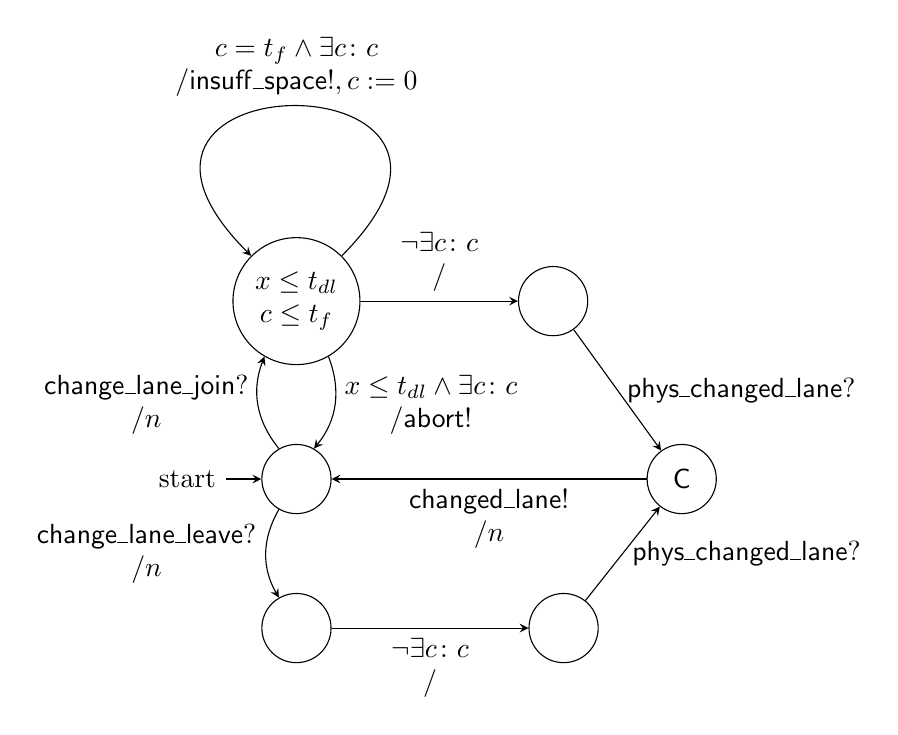
\begin{tikzpicture}[every text node part/.style={align=center}, >=stealth]
  \node[state, initial] (init) {};
  \node[state, above =of init] (join1) {\(x \leq t_{dl}\)\\\(c \leq t_f\)};
  \node[state, right=2cm of join1] (join2) {};
  \node[state, right=4cm of init] (wd1) {\textsf{C}};
  \node[state, below =of init] (leave1) {};
  \node[state, right=2.5cm of leave1] (leave2) {};

  \draw[->, bend left] (init) to node[ left, xshift=0cm] {\(\mathsf{change\_lane\_join?}\)\\ \(/\tclaim{\ego}{n} \)} (join1);
  \draw[->, bend left] (join1) to node[ right] {\(x \leq t_{dl} \land \exists c \colon \pcc{c} \)\\\(/\mathsf{abort!} \)} (init);
  \draw[->,loop] (join1) to node[above] {\(c = t_f \land \exists c \colon \pcc{c}\)\\\(/\mathsf{insuff\_space!}, c := 0 \)} (join1);
  \draw[->] (join1) to node[above] {\(\lnot \exists c \colon \pcc{c}\) \\ \(/ \treserve{\ego}\)} (join2);
  \draw[->] (join2) to node[right] {\(\mathsf{phys\_changed\_lane?}\)} (wd1);

  \draw[->, bend right] (init) to node[left] {\(\mathsf{change\_lane\_leave?}\)\\\(/\tclaim{\ego}{n}\)} (leave1);
  \draw[->] (leave1) to node[below] {\(\lnot \exists c \colon \pcc{c}\) \\ \(/ \treserve{\ego}\)} (leave2);
  \draw[->] (leave2) to node[right] {\(\mathsf{phys\_changed\_lane?}\)} (wd1);

  \draw[->] (wd1) to node[below] {\(\mathsf{changed\_lane!}\)\\\(/\twdreserve{\ego}{n}\)} (init);
\end{tikzpicture}

\paragraph{Ideas:}
\begin{itemize}
\item merging two platoons, i.e., joining several vehicles to one platoon 
(for a reference model check Grand Cooperative Driving Challenge - GCDC 
2016)
\begin{itemize}
\item parallel joining- we need some sort of assumption for joining vehicles.
Lets assume a joining vehicle always adjust its position reletice to the 
position of preceeding vehicle in the platooning
\item check Peleton technology for developing truck platooning tech.
\end{itemize}
\item thinking of other applications of spatial and real-time model
\end{itemize}

\end{document}



